\section{Linear Regression for Bivariate Data}

The Polynomial Basis Function used takes the form,

\begin{align*}
    \phi{(\mathbf{x})} &= \{\mathbf{x}_1^i \mathbf{x}_2^j\}
    \intertext{Where, $0 \leq i,j \leq Degree$ and $i+j \leq Degree$ In case of data points with two features, the polynomial basis functions includes,}
    \phi{(\mathbf{x})} &= \{ 1,\mathbf{x}_1, \mathbf{x}_2, \mathbf{x}_1^2, \mathbf{x}_2^2, \mathbf{x}_1\mathbf{x}_2, \mathbf{x}_1^{2}\mathbf{x}_1^{2} \}
\end{align*}


\subsection{Experiments $\And$ Observations on Dataset 2: }

\subsubsection{RMS comparison for varying regularisation parameter $\lambda$ (quadratic regularisation):}

Different $\lambda$ values were tested across different models with the goal of finding any $\lambda$ value that might be able to ameliorate any overfitting. However across all models, the increase of $\lambda$ value was accompanied with the strict increase of RMS value. Therefore, subsequent analysis has been carried out without regularization. The best model which was found to be of $batch = 500$ and $degree = 6$ with no regularisation performed with significant accuracy on the training, test and cross validation without any instances of overfitting. The effect of $\lambda$ is illustrated in the figure[\ref{fig:11}]. The table[\ref{table:3}] illustrates the analysis of different $\lambda$ values across the $degree= 6$ model and it can be inferred without doubt from the table that the best fitting model has $\lambda = 0$.

{\rowcolors{3}{green!40!yellow!10}{green!0!yellow!30}
\begin{table}[!ht]
\centering
\scalebox{0.80}{\begin{tabular}{ |p{1.0cm}|p{3.5cm}|p{3.5cm}| p{3.5cm}|  }
\hline
\multicolumn{4}{|c|}{$\mathbf{E}_{rms}$ values for different data } \\
\hline
\rowcolor{lightgray} \textbf{$\lambda$} & $\mathbf{E}_{rms-train}$ & $\mathbf{E}_{rms-test}$ & $\mathbf{E}_{rms-valid}$ \\
\hline
 1   &   7.58e-06  &  1.06e-05   &  7.51e-06   \\   
 \hline
 0   &   1.21e-07   &   1.15e-07  &   1.17e-07         \\
 \hline
 0.1   &   7.75e-06   &    1.06e-06     &     7.77e-07     \\
 \hline
 0.01  &   1.04e-07    &    1.31e-07   &     1.01e-07    \\
 \hline
 0.001  &   1.18e-07  &    1.08-07       &     1.17e-07      \\
 \hline
 0.0001  &   3.30e-08     &     3.2e-08      &      3.08e-08   \\
 \hline
 1e-05   &   1.77e-07    &     1.65e-07      &     1.69e-07  \\
\hline
\end{tabular}}
\caption{Error comparisons for varying values of $\lambda $ for Dataset 2 and a model of $degree = 6$}.
\label{table:4}
\end{table}
}


\begin{figure}[!ht]
    \centering
    \begin{subfigure}[t]{0.25\textwidth}
        \centering
        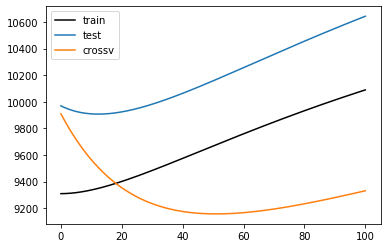
\includegraphics[height=1in]{Task 2 Images/batch500_deg2_lambda.png}
        \caption{Degree, $M = 2$}
    \end{subfigure}%
    ~ 
    \begin{subfigure}[t]{0.25\textwidth}
        \centering
        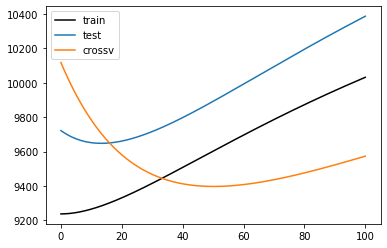
\includegraphics[height=1in]{Task 2 Images/batch500_deg3_lambda.png}
        \caption{Degree, $M = 3$ }
    \end{subfigure}%
    ~
    \begin{subfigure}[t]{0.25\textwidth}
        \centering
        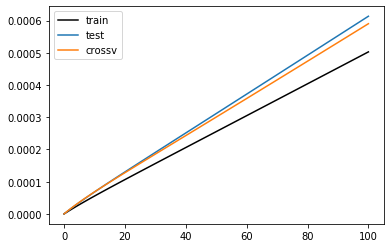
\includegraphics[height=1in]{Task 2 Images/batch500_deg6_lambda1to100.png}
        \caption{ Degree, $M = 6$}
    \end{subfigure}
    \caption{Effect of $\lambda$}
    \label{fig:11}
\end{figure}





\subsubsection{RMS comparison across different models}

Tables [\ref{table:5}], [\ref{table:6}], [\ref{table:7}], and [\ref{table:8}] provides an error based analysis of the model implemented.

{\rowcolors{3}{green!40!yellow!10}{green!0!yellow!30}
\begin{table}[!h]
\begin{tabular}{ |p{1.5cm}|p{3cm}|p{3cm}| p{3cm}|  }
\hline
\multicolumn{4}{|c|}{$\mathbf{E}_{rms}$ values for different data } \\
\hline
\rowcolor{lightgray} Degree & $\mathbf{E}_{rms-train}$ & $\mathbf{E}_{rms-test}$ & $\mathbf{E}_{rms-valid}$ \\
\hline
 2   &   8472.09  &  7916.24  &  11603.31   \\   
 \hline
 3   &   7746.87   &   10209.22  &   9055.03   \\
 \hline
 6   &   1.11e-06   &    7.12e-06     &     1.032e-06    \\
\hline
\end{tabular}
\caption{Error comparisons for varying degrees $\phi(\mathbf{x}) $ for Dataset 2 using 50 samples}.
\label{table:5}
\end{table}

\begin{table}[!h]
 \vspace*{\floatsep}
 \begin{tabular}{ |p{1.5cm}|p{3cm}|p{3cm}| p{3cm}|  }
\hline
\multicolumn{4}{|c|}{$\mathbf{E}_{rms}$ values for different data } \\
\hline
\rowcolor{lightgray} Degree & $\mathbf{E}_{rms-train}$ & $\mathbf{E}_{rms-test}$ & $\mathbf{E}_{rms-valid}$ \\
\hline
 2   &   7836.93  &  9102.67 &  10203.59  \\   
 \hline
 3   &   7410.93  &   8955.31 &   9615.30    \\
 \hline
 6   &   9.07e-08   &    1.14e-07     &     9.06e-08    \\
\hline
\end{tabular}
\caption{Error comparisons for varying degrees $\phi(\mathbf{x}) $ for Dataset 2 using 100 samples}.
\label{table:6}
\end{table}

\begin{table}[!h]
\vspace*{\floatsep}
 \begin{tabular}{ |p{1.5cm}|p{3cm}|p{3cm}| p{3cm}|  }
\hline
\multicolumn{4}{|c|}{$\mathbf{E}_{rms}$ values for different data } \\
\hline
\rowcolor{lightgray} Degree & $\mathbf{E}_{rms-train}$ & $\mathbf{E}_{rms-test}$ & $\mathbf{E}_{rms-valid}$ \\
\hline
 2   &   9007.85  &  9941.50 & 7712.90   \\   
 \hline
 3   &   8891.04   &   10448.97  &   7669.04    \\
 \hline
 6   &   2.77e-08   &    3.15e-08     &     3.17e-08   \\
\hline
\end{tabular}
\caption{Error comparisons for varying degrees $\phi(\mathbf{x}) $ for Dataset 2 using 200 samples}.
\label{table:7}
\end{table}

\begin{table}[!ht]
\vspace*{\floatsep}
 \begin{tabular}{ |p{1.5cm}|p{3cm}|p{3cm}| p{3cm}|  }
\hline
\multicolumn{4}{|c|}{$\mathbf{E}_{rms}$ values for different data } \\
\hline
\rowcolor{lightgray} Degree & $\mathbf{E}_{rms-train}$ & $\mathbf{E}_{rms-test}$ & $\mathbf{E}_{rms-valid}$ \\
\hline
 2   &   9308.74  &  9968.55 & 9908.81   \\   
 \hline
 3   &   9237.93   &   9721.98  &   10117.44    \\
 \hline
 6   &   2.54e-08   &    2.92e-08     &     2.51e-08  \\
\hline
\end{tabular}
\caption{Error comparisons for varying degrees $\phi(\mathbf{x}) $ for Dataset 2 using 500 samples}.
\label{table:8}
\end{table}
}


\newpage
\subsubsection{Surface Plots with Training set superimposed}
Figures [\ref{fig:12}], [\ref{fig:13}], [\ref{fig:14}] and [\ref{fig:15}] are the various surface plots.

\begin{figure}[!ht]
    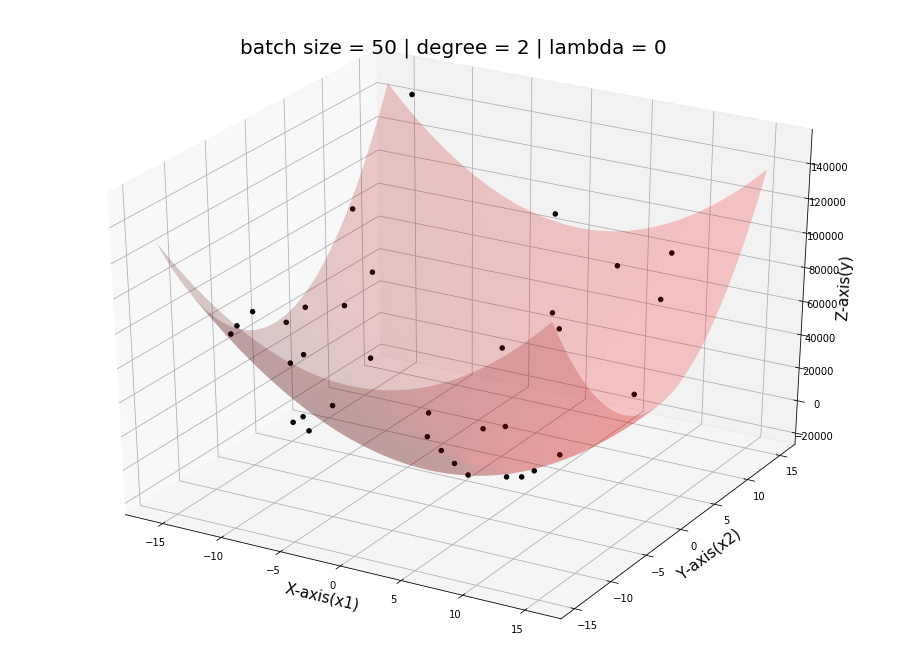
\includegraphics[width=.30\textwidth]{Task 2 Images/surfaceplot_batch50_deg2_lamb0.png}\hfill
    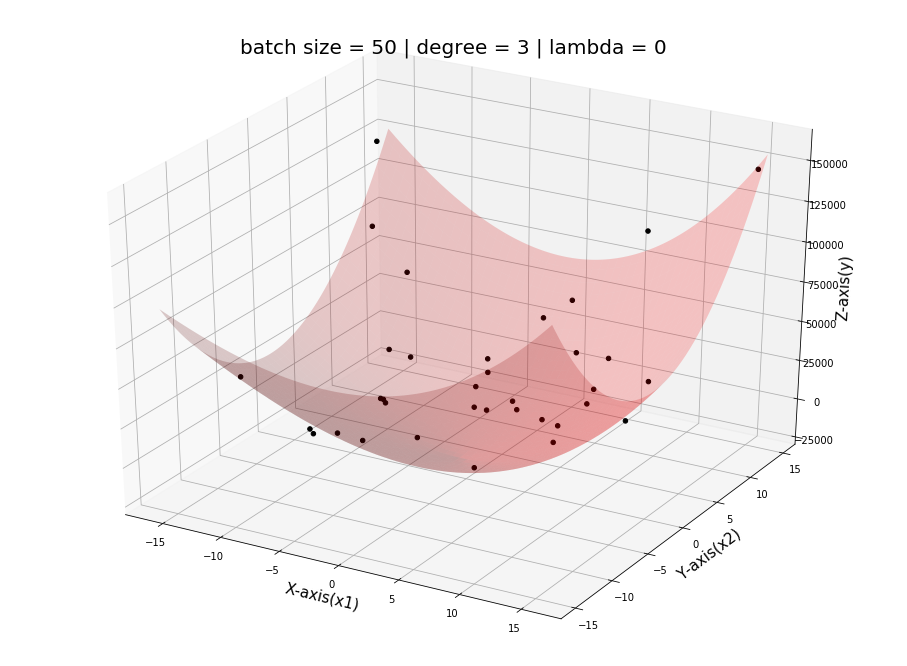
\includegraphics[width=.30\textwidth]{Task 2 Images/surfaceplot_batch50_deg3_lamb0.png}\hfill
    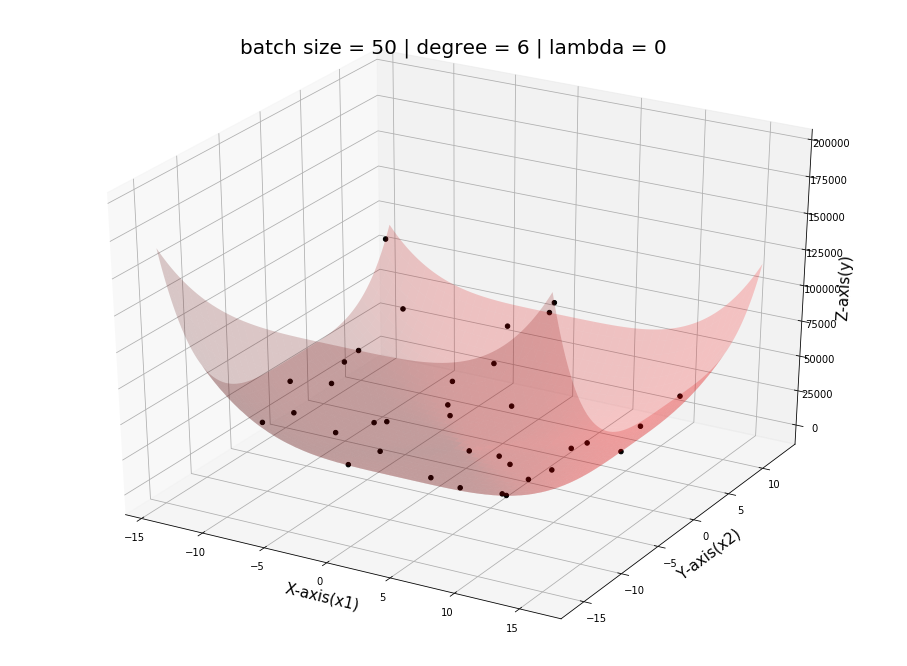
\includegraphics[width=.30\textwidth]{Task 2 Images/surfaceplot_batch50_deg6_lamb0.png}
    \caption{Surface Plots using various degree for a fixed best regularisation parameter $\lambda = 0$ using 50 samples }
    \label{fig:12}
\end{figure}

\begin{figure}[!ht]
    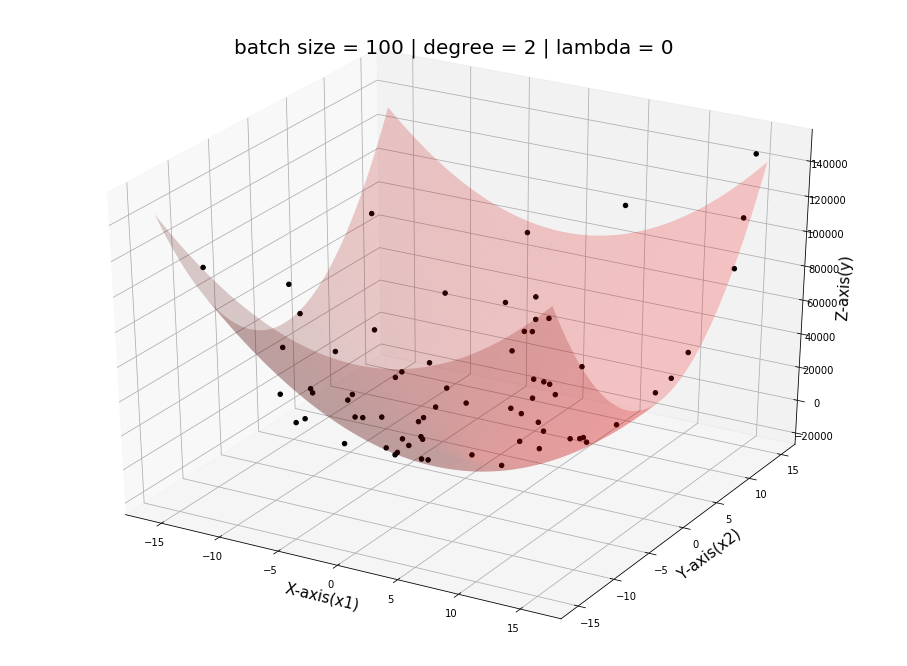
\includegraphics[width=.30\textwidth]{Task 2 Images/surfaceplot_batch100_deg2_lamb0.png}\hfill
    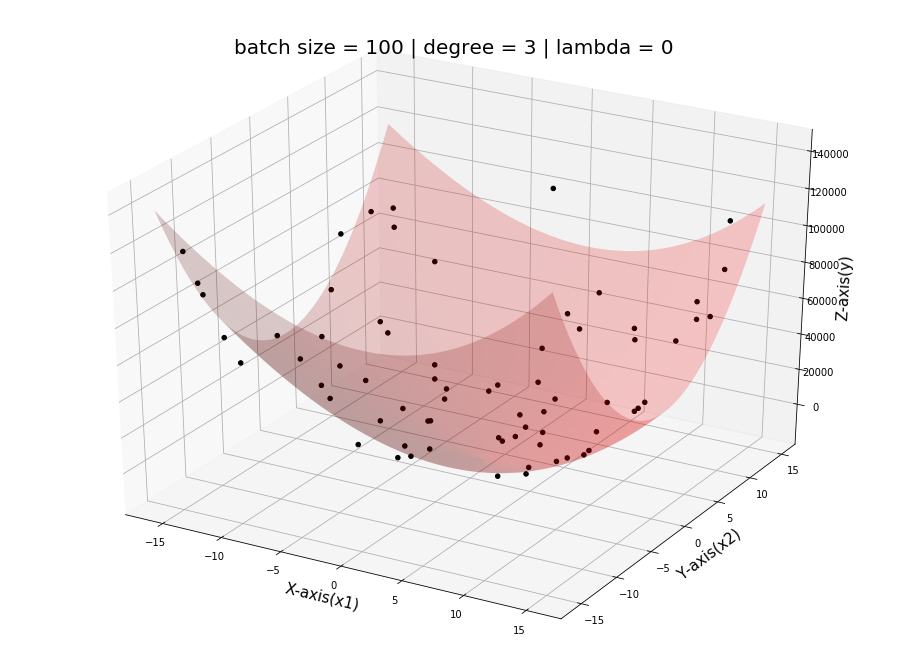
\includegraphics[width=.30\textwidth]{Task 2 Images/surfaceplot_batch100_deg3_lamb0.png}\hfill
    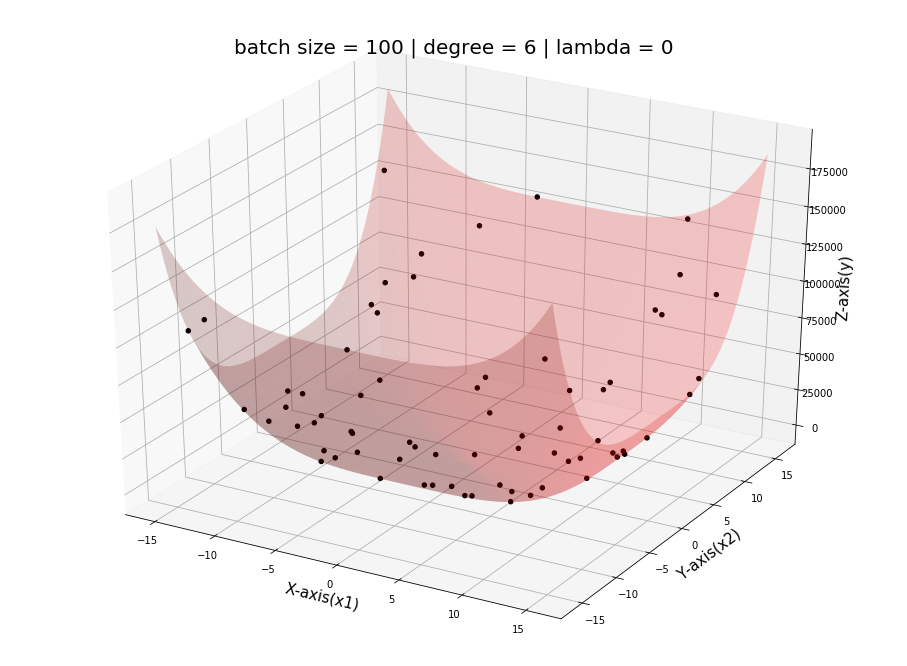
\includegraphics[width=.30\textwidth]{Task 2 Images/surfaceplot_batch100_deg6_lamb0.png}
    \caption{Surface Plots using various degree for a fixed regularisation parameter $\lambda = 0$ using 100 samples}
    \label{fig:13}
\end{figure}

\begin{figure}[!ht]
    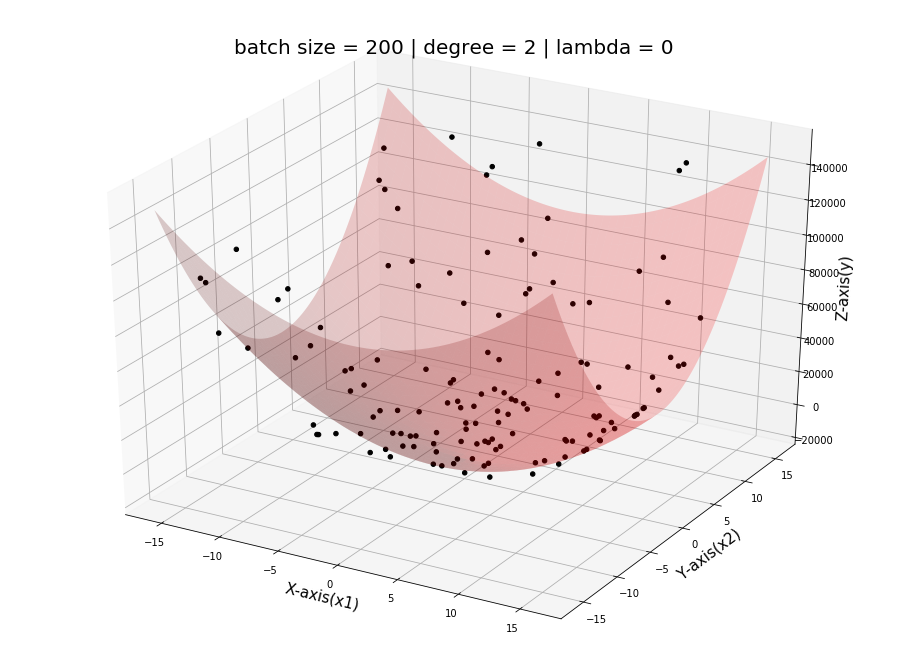
\includegraphics[width=.30\textwidth]{Task 2 Images/surfaceplot_batch200_deg2_lamb0.png}\hfill
    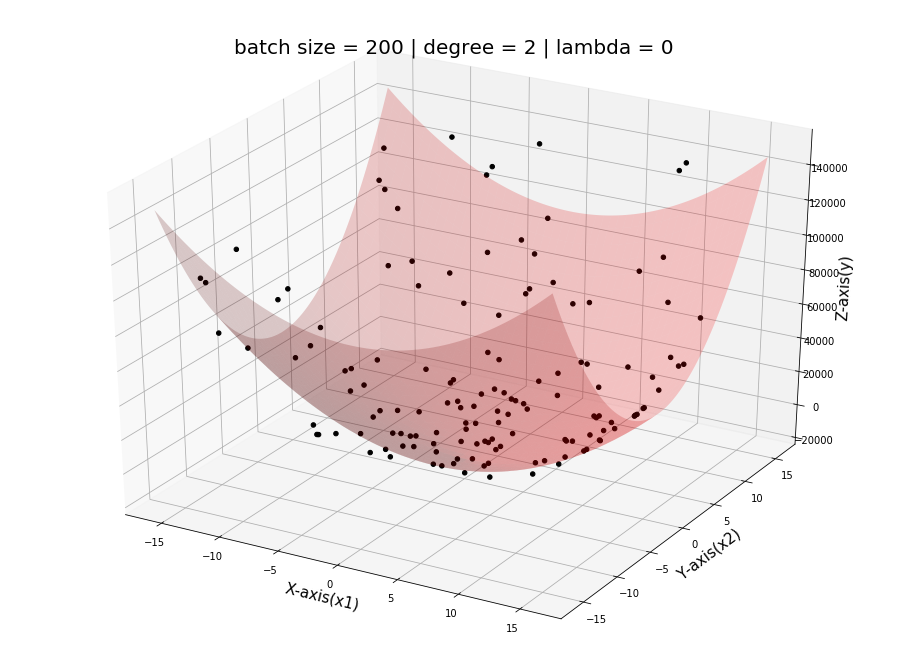
\includegraphics[width=.30\textwidth]{Task 2 Images/surfaceplot_batch200_deg2_lamb0.png}\hfill
    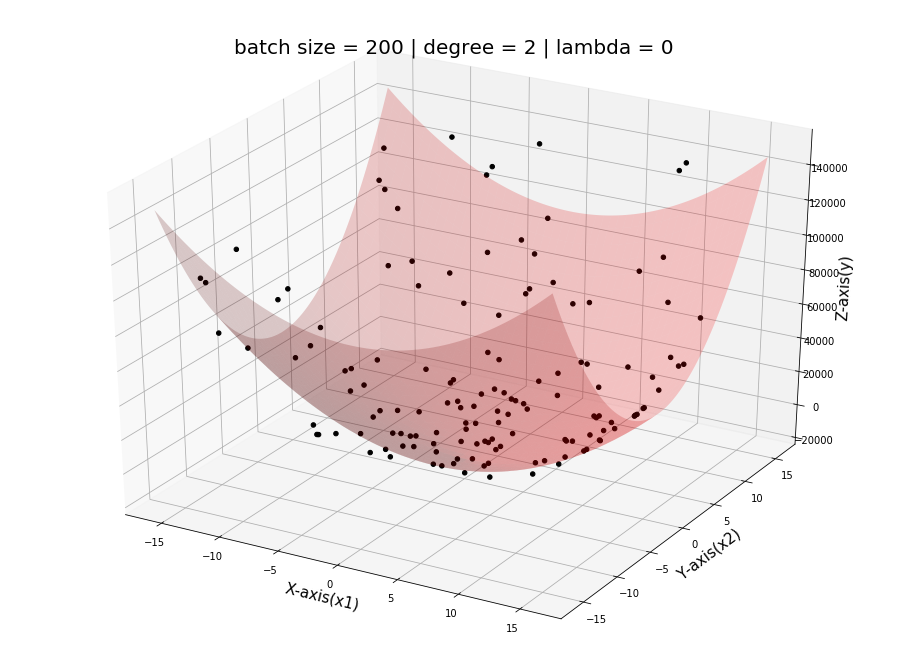
\includegraphics[width=.30\textwidth]{Task 2 Images/surfaceplot_batch200_deg2_lamb0.png}
    \caption{Surface Plots using various degree for a fixed regularisation parameter $\lambda = 0$ using 200 samples}
    \label{fig:14}
 \end{figure}


\begin{figure}[!ht] 
    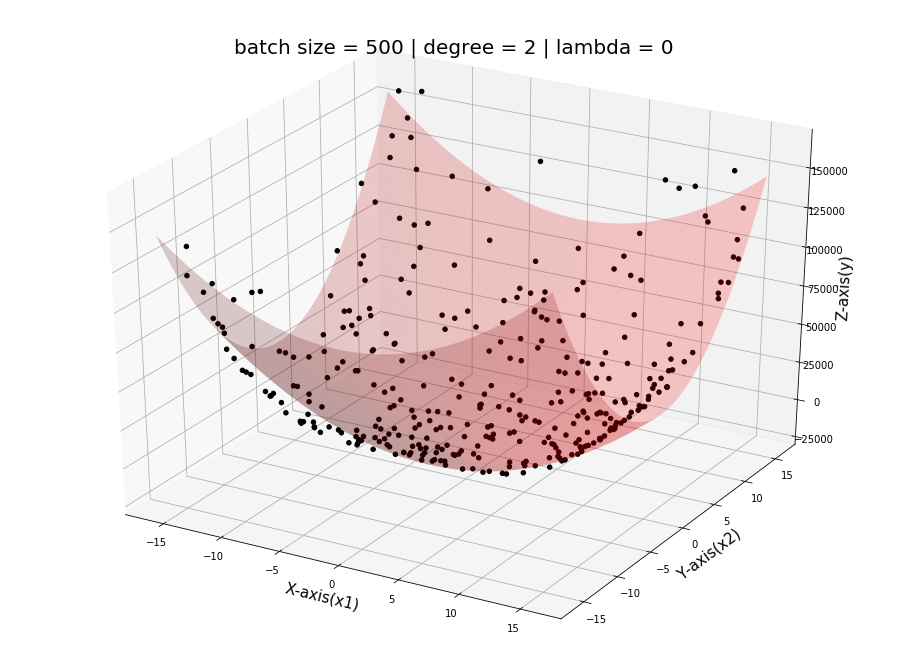
\includegraphics[width=.30\textwidth]{Task 2 Images/surfaceplot_batch500_deg2_lamb0.png}\hfill
    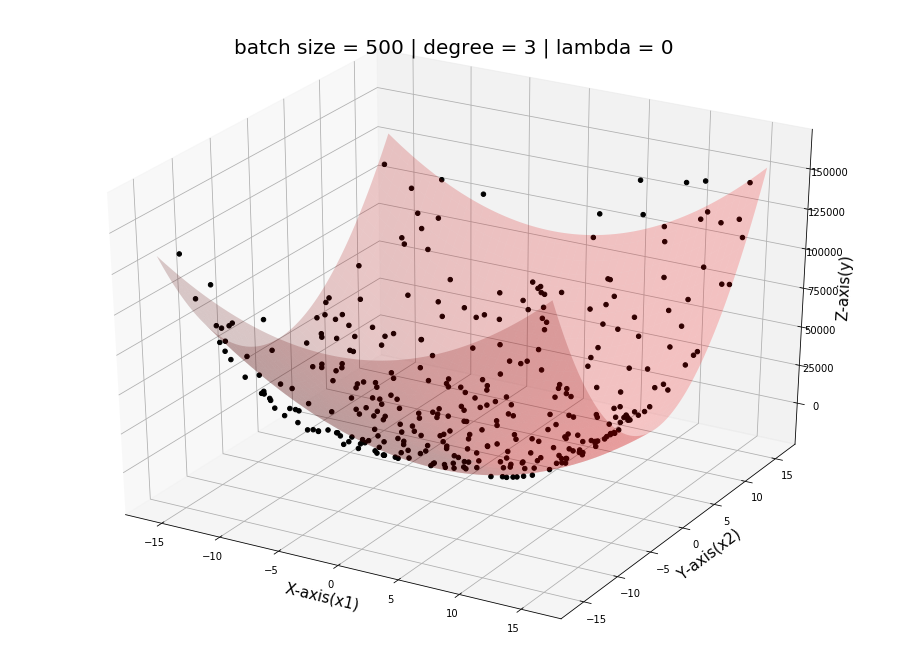
\includegraphics[width=.30\textwidth]{Task 2 Images/surfaceplot_batch500_deg3_lamb0.png}\hfill
    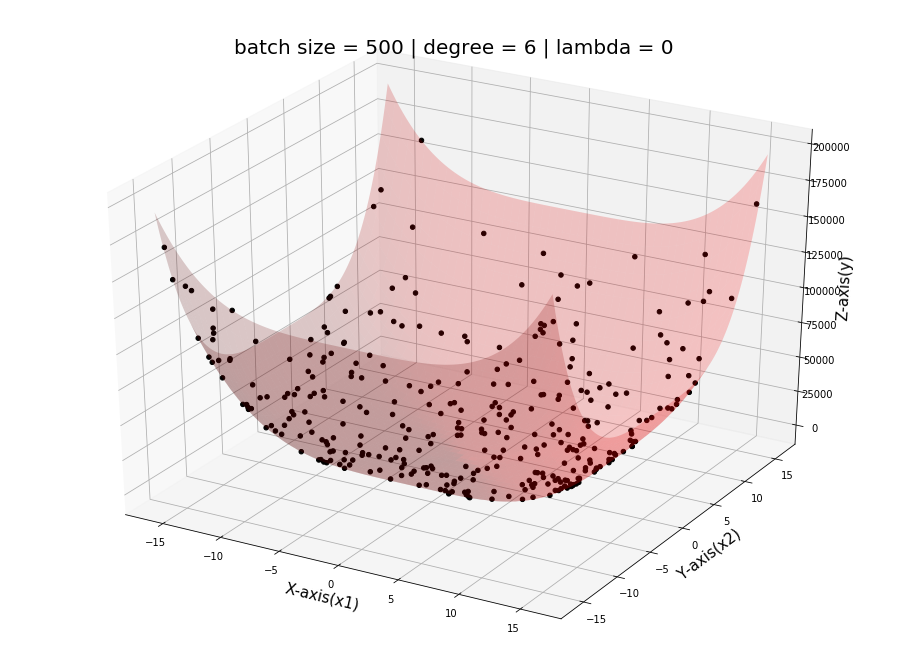
\includegraphics[width=.30\textwidth]{Task 2 Images/surfaceplot_batch500_deg6_lamb0.png}
    \caption{Surface Plots using various degree for a fixed regularisation parameter $\lambda = 0$ using 500 samples}
    \label{fig:15}
\end{figure}

\newpage
\subsubsection{Scatter Plots of the Best Model}
The best model was found to be of batch size 500 and degree 6 without any regularization and fared significantly better than the other degree 2,3 models as it's $E_{rms}$ values were found to be smaller in orders of magnitude $10^9$. Scatter plots of the best model are represented in figure [\ref{fig:16}]


 \begin{figure}[!ht]
     \centering
     \begin{subfigure}[t]{0.30\textwidth}
         \centering
         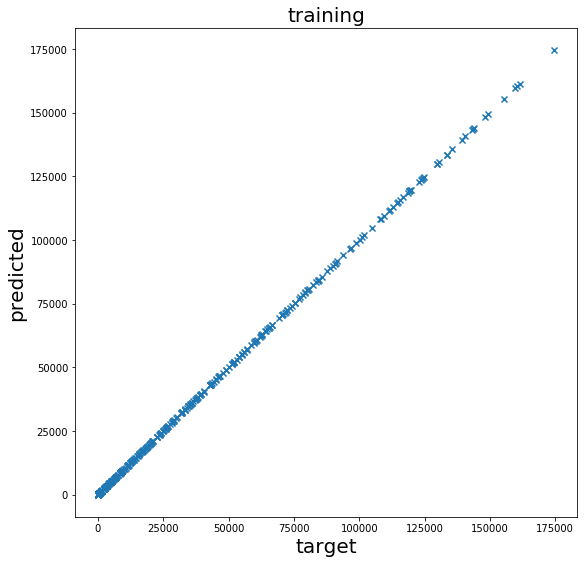
\includegraphics[height=1.6in]{Task 2 Images/best_scatterplot_batch_500_degree_6_lambda_0_training.png}
         \caption{Training Data}
     \end{subfigure}%
     ~ 
     \begin{subfigure}[t]{0.30\textwidth}
         \centering
         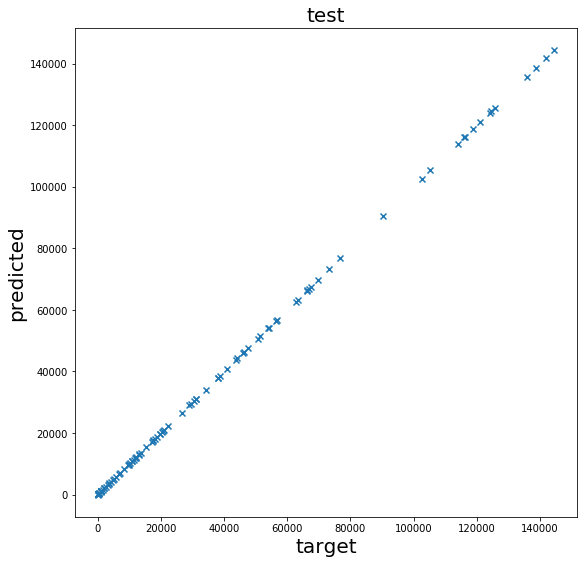
\includegraphics[height=1.6in]{Task 2 Images/best_scatterplot_batch_500_degree_6_lambda_0_test.png}
         \caption{Test Data }
     \end{subfigure}%
     ~
     \begin{subfigure}[t]{0.30\textwidth}
         \centering
         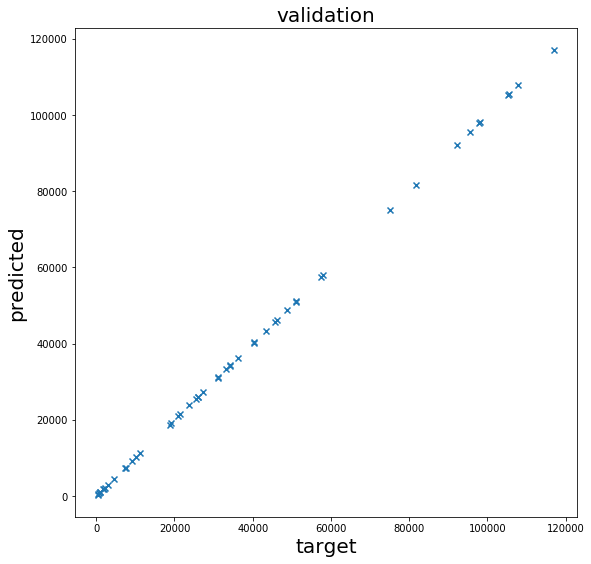
\includegraphics[height=1.6in]{Task 2 Images/best_scatterplot_batch_500_degree_6_lambda_0_validation.png}
         \caption{Validation Data }
     \end{subfigure}
     \caption{Best Scatter Plot}
     \label{fig:16}
\end{figure}
